\documentclass[10pt,twocolumn,letterpaper]{article}

\usepackage{cvpr}
\usepackage{times}
\usepackage{epsfig}
\usepackage{graphicx}
\usepackage{amsmath}
\usepackage{amssymb}

% Include other packages here, before hyperref.

% If you comment hyperref and then uncomment it, you should delete
% egpaper.aux before re-running latex.  (Or just hit 'q' on the first latex
% run, let it finish, and you should be clear).
\usepackage[breaklinks=true,bookmarks=false]{hyperref}

\cvprfinalcopy % *** Uncomment this line for the final submission

\def\cvprPaperID{****} % *** Enter the CVPR Paper ID here
\def\httilde{\mbox{\tt\raisebox{-.5ex}{\symbol{126}}}}

% Pages are numbered in submission mode, and unnumbered in camera-ready
%\ifcvprfinal\pagestyle{empty}\fi
\setcounter{page}{1}

\begin{document}

\title{Human Pose Estimation for Video Game Control}
\author{Rakesh Johny, Tom Li, Aditya Narayanan, Albert Xia}
\maketitle

\begin{abstract}
    Current methods of interacting with computers are flawed in a 
    couple of key ways: they fail to map physically-intuitive motions to their computer 
    control counterparts, and they rely heavily on a user's fine-motor skills, 
    which are heavily impacted by factors such as muscle coordination disabilities 
    and old age. In this paper, we propose a system of computer control through 
    gesture tracking via real-time human pose estimation on an embedded device, 
    which is capable of addresssing these issues, by mapping general physically-intuitive 
    motions into computer control. Furthermore, our device boasts low latency in 
    the human-computer interaction, and is minimally intrustive to the computer being 
    controlled. We test the viability of our system as a computer-control device by playing two 
    video games using only gestures.
\end{abstract}

\section{Introduction}
The human-computer interfaces behind many modern video games use either handheld 
joystick controllers or keyboard and mouse input, which are examples
of typical human input device for computers, monitors, televisions, etc. There are two 
major drawbacks to traditional human input systems that are often overlooked: the input needed 
to achieve a certain effect has little to no correspondence to a physically-intuitive set 
of motions, and more importantly, inputs are heavily dependent on the user's fine motor skills. 
Fine motor skills used to interact with modern technology are heavily affected by factors such 
as muscular coordination disorders and old age. Computer vision, particularly the processes 
of human pose estimation and motion tracking may allow us to create human-computer interfaces 
that link computer control to physically-intuitive human motion inputs with little dependence on 
fine motor ability or additional physical input devices. We propose a vision-based computer-input 
system that maps gestures and motion of the user's body into computer input. We test the system's 
effectiveness with the playability of two simple video games as metrics. In order to demonstrate 
the versatility of our phased-approach to gesture-based control, we select a car-racing game and 
the Google Chrome Dino Racer game as test video games. Such a system, when expanded to replicating 
general keyboard + mouse control, would be instrumental in improving the accessibility of 
modern technology, with implementations far beyond the scope of computer games.

\section{Related Work}
\subsection{Human Pose Estimation}
Some of the largest components of our system fall into the category of so called Human 
Pose Estimation or the ability to properly:

\begin{itemize}
    \item Identify users as sources of input, from a video stream
    \item Segment the user's body to isolate relevant portions of data
    \item Compute location information about the user's body from relevant portions of data.
\end{itemize}

The area of Human Pose Estimation is widely studied. Robust, optimized solutions exist 
that can help us with this step. One popular solution is derived from \cite{8765346} which uses Part Affinity Fields (PAFs) to learn to assosciate body parts with individuals in the image, and 
open-source code for the so called openpose library shows promising results for real-time 
human body segmentation. 

\begin{figure}[h]
    \centering
    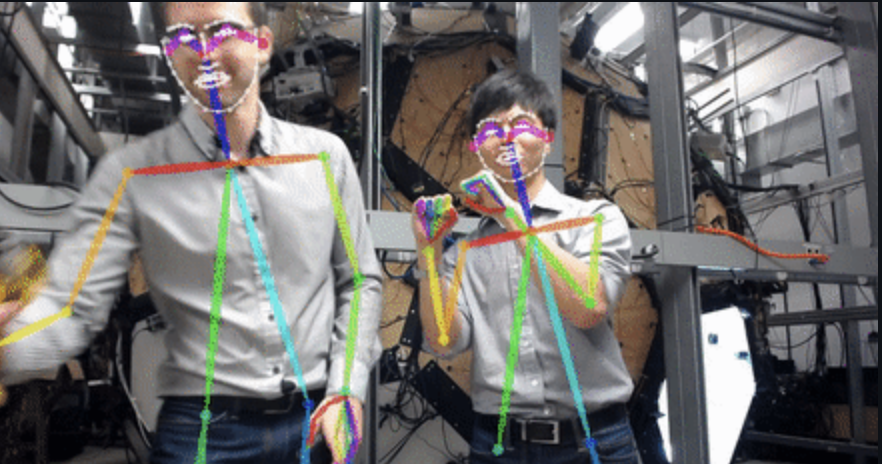
\includegraphics[width = .8\linewidth]{images/openpose.png}
    \caption{A demonstration of openpose performing human body segmentation.}
\end{figure}

\subsection{Gesture Identification/Motion Tracking}
\cite{8765346} and Openpose give us promising ways to identify locations of human body features 
(hands, arms, etc.) in a video stream. However, this is not enough to categorize a user's motion 
as a particular input. To be able to extract feature motion over time as a useful input to our 
car racing video game, we will have to implement motion tracking over a video stream. 

A number of guides exist for implementing feature tracking over video. \cite{tracking_1} 
and \cite{tracking_2} demonstrate simple object tracking across video frames, and \cite{tracking_2} 
demonstrates a system shown to be accurate with motion of hands. Implementing a similar system for 
tracking arbitrary features of the human body obtained from human pose estimation should provide 
adequate results.

\section{Methodology}
Our human computer interface will consist of three major steps: Pose Estimation, or feature 
location, Feature Tracking and classification of motions, and video game interfacing. Each one 
is detailed below. All code will be written in Python.

\subsection{Pose Estimation}
The first step of our human computer interface pipeline is the pose estimation step, in which 
we use openpose to locate certain key features of the user. What constitutes a key feature will 
be determined when the set of video game controls we must mimic is properly defined. Possible 
key features include the location of the user's wrists, elbows, or the angles of various limbs. 

During this step we will also determine the computational cost of openpose and make decisions on 
how to proceed based on the results. If openpose is able to run with sufficiently low latency, we 
move on to feature tracking, but if openpose demonstrates a high latency, we will explore other 
methods of pose estimation, or methods of improving the performance of openpose using by decreasing 
framerates or image resolutions.

\subsection{Feature Tracking}
Obtaining the locations of various important features is only the first step towards identifying 
physically-meaningful actions of the user. In order for the user to be able to signal various 
commands within the video game, we must track the previously obtained features over time and 
classify the user's behavior into one of a few possible actions. For example, mimicing a car 
racing game, the set of possible actions could be \{No command, accelerate, decelerate, steer\}. 
Each of these commands or classifications will also have a value associated with it corresponding 
to its magnitude, which will also be obtained directly from feature locations. For example, a steering 
command mapped to the user rotating their torso would have a steering value associated with it 
derived from the angle through which the user has turned. 

\subsection{Game Interface}
The third and final major step of our methodology is to turn the classifications obtained from 
the Feature Tracking step and feed them to a video game as user input. We will simply map each 
corresponding classification from step 2 to an "intermediate control" which is simply the 
joystick/keyboard/mouse input that would produce the same output from the game, and implement 
simple keyboard control with Python to feed that input to the video game.

\section{Results}

\section{Future Works}

{\small
\bibliographystyle{ieee_fullname}
\bibliography{proposal_bib}
}

\end{document}